\chapter{Administrer l'application}

\section{Gérer les droits}
\label{droits}

\subsection{Principe général}

Les droits sont gérés selon le principe initialement utilisé dans la bibliothèque PHPGACL, aujourd'hui obsolète. 

Les logins sont déclarés dans des groupes organisés de manière hiérarchique : un groupe hérite des droits attribués à ses parents.

Les droits utilisés dans le logiciel sont associés à des groupes. Il est possible d'attribuer plusieurs droits à un même groupe, et un droit peut être détenu par des groupes différents.

Si le paramètre \textit{\$LDAP["groupSupport"]} est positionné à \textit{true}, les groupes dont fait partie le compte LDAP sont également récupérés, et peuvent être détenteurs de droits dans le logiciel (le nom des groupes est sensible à la casse).

Voici le schéma des tables utilisées pour gérer les droits :

\begin{figure}[H]
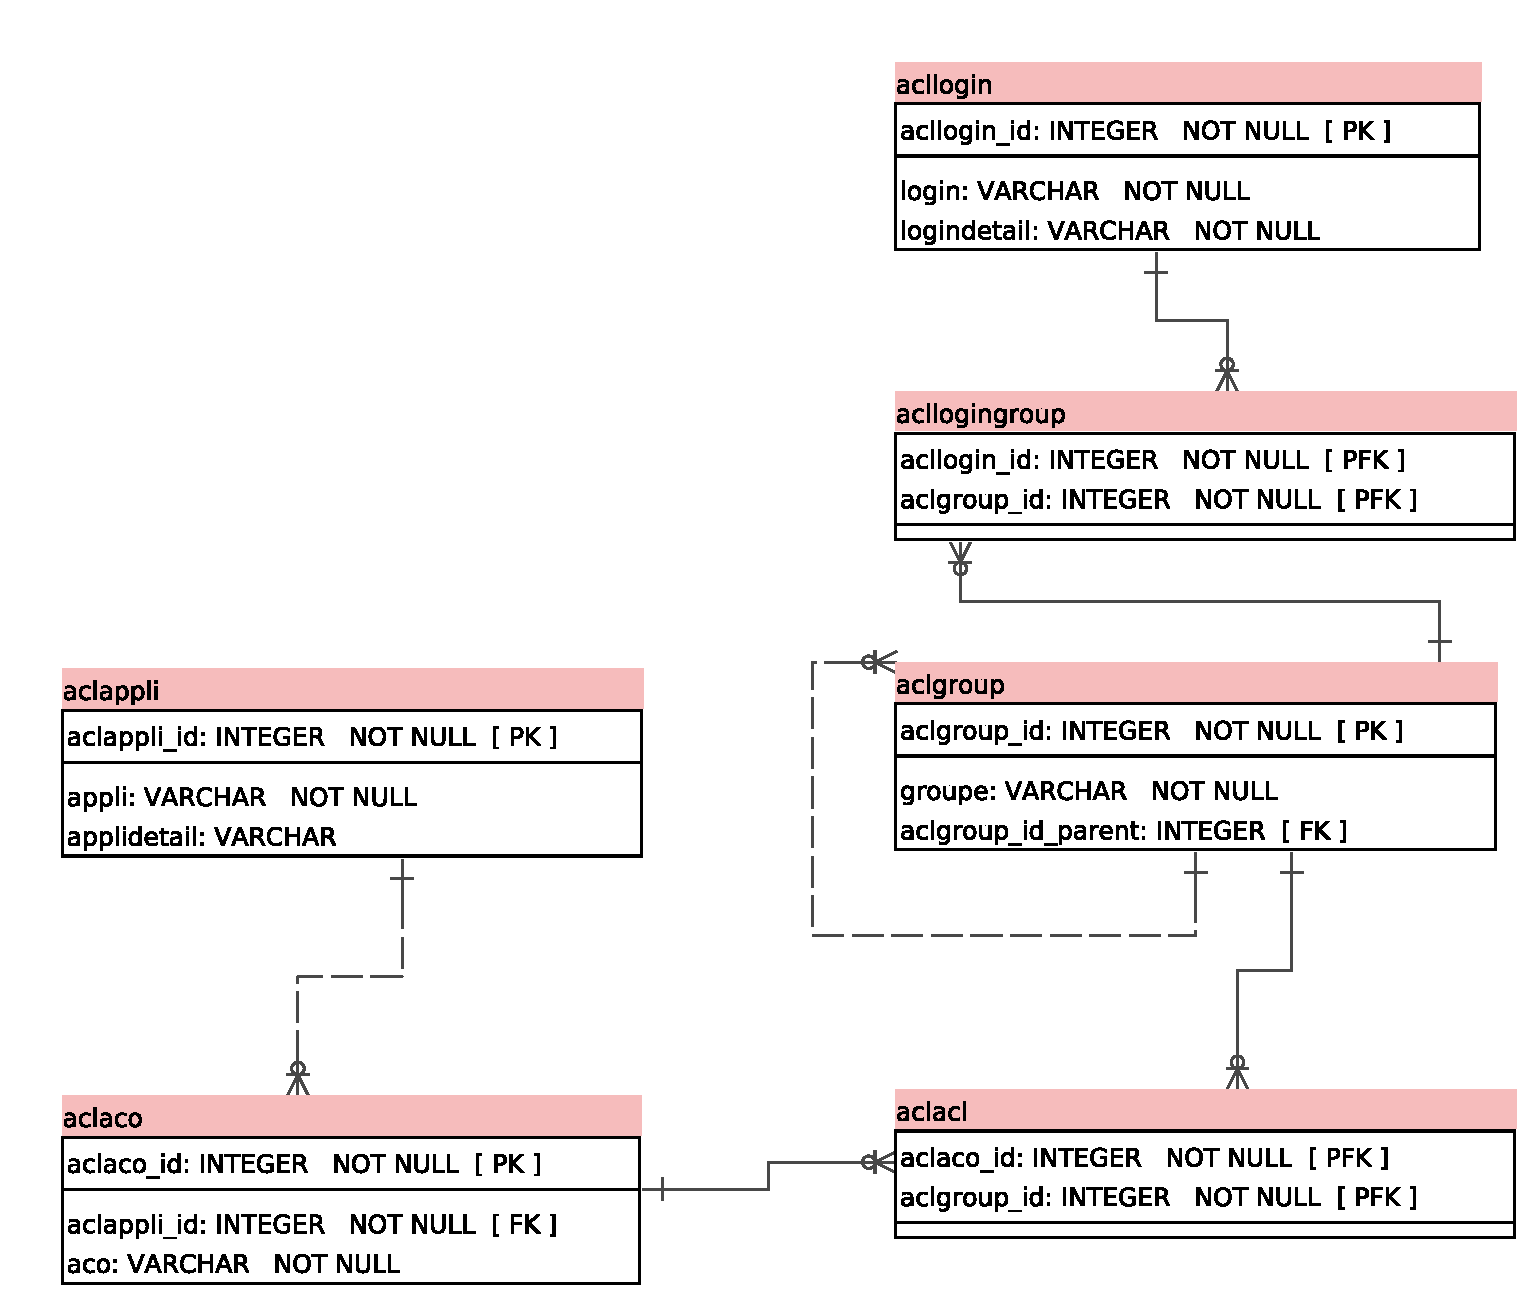
\includegraphics[width=\linewidth]{images/acl_only}
\caption{Schéma des tables utilisées pour gérer les droits}
\end{figure}

Voici la description des tables :
\begin{description}
\item[acllogin] Liste des logins utilisés. Si un compte est créé dans la base locale d'identification, un enregistrement est également créé dans cette table. Pour les identifications LDAP ou CAS, ils doivent être identiques. Si seuls les groupes LDAP sont utilisés pour un compte, il n'a pas besoin d'être décrit ici
\item[aclappli] Liste des applications gérées. Il est ainsi possible de gérer, à partir de la même base de données, plusieurs ensembles de droits, qui utilisent les mêmes logins
\item[aclaco] liste des droits déclarés dans l'application
\item[aclgroup] Liste des groupes contenant les logins, et qui détiennent les droits. Un groupe peut hériter d'un autre groupe. Les droits associés au groupe parent sont également attribués au groupe hérité.
\item[acllogingroup] table permettant de déclarer les logins associés à un groupe
\item[aclacl] table décrivant les droits détenus par un groupe
\end{description}

Le module d'administration permet de saisir toutes ces informations. Il faut que l'utilisateur dispose du droit \textit{admin}, c'est à dire faire partie du groupe \textit{admin} (configuration par défaut à l'initialisation de la base des droits) pour pouvoir accéder à ces fonctions.

\subsection{Droits à positionner}
Voici les groupes nécessaires pour faire fonctionner correctement l'application :

\begin{longtable}{|p{5cm}|p{10cm}|}
\hline
\textbf{Droit} & \textbf{Usage} \\
\hline
\endhead
admin &	Gestion des utilisateurs et des droits\\
\hline
param &	Définition des tables de paramètres généraux, Gestion d'un projet\\
\hline
projet &	rajout des types d'échantillons ou de conteneurs, import de masse \\
\hline
gestion &	Ajout d'un échantillon pour les projets autorisés, entrée/sortie. Droit attribué par défaut si l'utilisateur fait partie d'au moins un projet \\
\hline
consult	& Consultation des informations, sans possibilité de modification. Le droit de consultation doit être indiqué volontairement\\
\hline
\caption{Liste des droits utilisés}
\end{longtable}

\subsection{Gestion des projets}

Les échantillons doivent être rattachés à un projet, vous devrez en créer au minimum un à partir du menu d'administration. Un utilisateur avec les droits de gestion ne peut modifier que les échantillons pour lesquels il est autorisé (les projets qui sont rattachés au groupe dont il fait partie).

Voici le principe de gestion des droits pour les projets :

Dans \textit{Administration} > \textit{ACL - Groupes de logins}, déclarez les groupes adéquats. En cas d'utilisation des groupes LDAP, les saisir avec la même casse que dans l'annuaire (EABX p. e.).

Il est possible de définir une hiérarchie des groupes, quelle que soit l'origine de l'affectation (base de données ou annuaire Ldap)
Dans le cas où l'annuaire Ldap n'est pas utilisé pour gérer les groupes, renseignez les logins en face des groupes dans le même écran.

Dans les projets, sélectionnez les groupes autorisés.